\documentclass{sigchi}
\pagenumbering{arabic}


% Load basic packages
\usepackage{balance}  % to better equalize the last page
\usepackage{graphics} % for EPS, load graphicx instead
\usepackage{times}    % comment if you want LaTeX's default font
\usepackage{url}      % llt: nicely formatted URLs

% llt: Define a global style for URLs, rather that the default one
\makeatletter
\def\url@leostyle{%
  \@ifundefined{selectfont}{\def\UrlFont{\sf}}{\def\UrlFont{\small\bf\ttfamily}}}
\makeatother
\urlstyle{leo}


% To make various LaTeX processors do the right thing with page size.
\def\pprw{8.5in}
\def\pprh{11in}
\special{papersize=\pprw,\pprh}
\setlength{\paperwidth}{\pprw}
\setlength{\paperheight}{\pprh}
\setlength{\pdfpagewidth}{\pprw}
\setlength{\pdfpageheight}{\pprh}

% Make sure hyperref comes last of your loaded packages, 
% to give it a fighting chance of not being over-written, 
% since its job is to redefine many LaTeX commands.
\usepackage[pdftex]{hyperref}
\hypersetup{
pdftitle={DuoDrive},
pdfauthor={LaTeX},
pdfkeywords={SIGCHI, proceedings, archival format},
bookmarksnumbered,
pdfstartview={FitH},
colorlinks,
citecolor=black,
filecolor=black,
linkcolor=black,
urlcolor=black,
breaklinks=true,
}

% create a shortcut to typeset table headings
\newcommand\tabhead[1]{\small\textbf{#1}}


% End of preamble. Here it comes the document.
\begin{document}

\title{DuoDrive}

\numberofauthors{2}
\author{
  \alignauthor Ramin Erfani, Kevin van Nes, Robert Luijendijk, Pim van den Bogaerdt, Mourad el Maouchi\\
    \affaddr{Delft University of Technology}\\
    \affaddr{Delft, The Netherlands}\\
    \email{erfani.ramin@gmail.com, kevinvnes@gmail.com, luijendijk12@gmail.com, pimvandenbogaerdt@hotmail.com, mourad.tudelft@elmaouchi.com}\\
  \alignauthor Bastiaan Anthonie Reijm\\
    \affaddr{Delft University of Technology}\\
    \affaddr{Delft, The Netherlands}\\
    \email{reijm.bastiaan@gmail.com}\\
}

\maketitle

\begin{abstract}
In this paper we describe our game DuoDrive
which is a racing game where two teams of
two players each control one car and try to
reach the finish. This document outlines a brief
description about the features of this game, the target
audience we chose and the technological and
game play innovations. DuoDrive was developed
for Android.
\end{abstract}

\keywords{
	Student game design competition; Mobile game; race; multiplayer;
}

\section{Introduction}

We wanted a game that would force interaction, real communication between players which involved a lot of humor and entertainment. We therefore developed DuoDrive, a game that can be classified as a race game which ensures a lot of communication and interaction. The main idea behind the game is to divide a classical car driver into two parts: a driver and a throttler. In real life these two parts are controlled by one person, by splitting these, a lot of cooperation needs to be done. Not only to reach the finish, but to make sure you're going to win.

\section{Game overview}

In this game people have to play against each other in pairs, sort of like tag-teams. The race consists of two cars, each car having two players, for a total of four players. Both players controlling a car have to cooperate to reach the finish. As the driver: the player that controls the steering, cannot see beyond his own headlights. As for the throttler: the player can only see an overview of the track but cannot see obstacles on the track.

By having these two functions, both players in a team have to cooperate both physically and virtually. In order to take turns on time, the throttler has to physically inform the steerer to turn left or to turn right. In addition, the steerer will have to physically inform the throttler that he sees a slowdown warning as there is mud incoming or that he has to throttle backwards once the steerer collided in a turn.

These features are there to spice up a classical race game, our game is significantly more difficult than any other classical race game. However, this comes with an asset, amusement. 

\section{Target audience}

We did not implicitly target an audience, however we did keep in mind that it is mostly males that will take initiative to create a game. We also noted that 40+ people often have difficulty's with the game's controls, especially women. We therefore said that our main audience would be males aging between 14 - 30 years.

This audience mostly contains experienced gamers, it doesn't matter what genre they like, just playing games in general make players more experienced and thus will more appreciate our game.

\subsection{Technological and game play innovations}

Technically, we did not innovate at all. We used low-budget technology as Wi-Fi to let players virtually cooperate. We score our points on the game concept.\\\\
Our gameplay innovates in that there has never been a game before where driving a car has been split into two seperate handlings. And it innovates in the fact that our game enforces physical cooperation. Merely virtual cooperation will not get you anywhere near the lead.

\subsection{Game design}

We decided on creating a mobile game for Android using the Unity framework
because of it's widely accepted image, which in turn ensured a lot of tutorials
on which we could work on.

The software architecture of the system consists of three different subsystems: the server, the system for the steering player and the system for the player who controls the throttle.

\begin{itemize}
\item Server \hfill \\
    The server is a subsystem that maintains the data flow. For example, it will send the data of the positions of the cars to all players, so that every player has a near real-time experience, where they can see other players' positions. All data sent by a player will first be sent to the server, which distributes it to the other players. There is no player-to-player data flow at this moment.
\item Steering player system \hfill \\
    The system for the steering player will only contain the view that the steering player sees. This will be a limited view, as the steering player will only see a small area in front of his car. The steering player will also not be able to throttle. For a detailed picture of the interface of the steering player, see Figure \ref{fig:figure1}
\item Throttler system \hfill \\
    In the throttler system the ability to perform certain actions is also limited. The player will only be able to control the throttle, i.e. accelerating forward or backward and hitting the brake. By limiting the view and the possible actions, communication between the throttling player and steering player will be enforced.
\end{itemize}

We visually designed our game to be simple and clear. The interface contains limited possibility's to ensure that the players will quickly understand the use of each button.

\begin{figure}[!h]
\centering
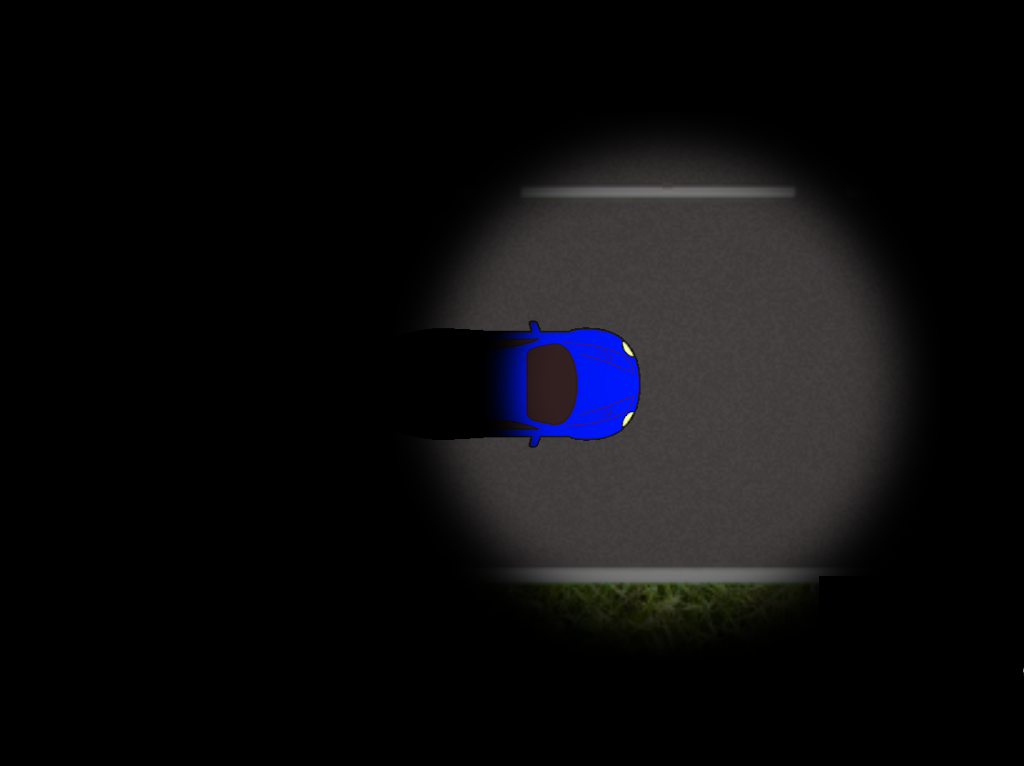
\includegraphics[width=0.9\columnwidth]{Figure1}
\caption{The interface of the steering player.}
\label{fig:figure1}
\end{figure}

\subsection{Game trailer}

We created a video showing the gameplay of DuoDrive.
Showing the most important aspects of the game and creating
a feeling of the game. It can be viewed here:

\subsection{Acknowledgements}

We would like to thank....

%\subsection{References and Citations}

%Use a numbered list of references at the end of the article, ordered
%alphabetically by first author, and referenced by numbers in brackets
%\cite{ethics,
%  Klemmer:2002:WSC:503376.503378,
%  Mather:2000:MUT,
%  Zellweger:2001:FAO:504216.504224}. For
%papers from conference proceedings, include the title of the paper and
%an abbreviated name of the conference (e.g., for Interact 2003
%proceedings, use \textit{Proc. Interact 2003}). Do not include the
%location of the conference or the exact date; do include the page
%numbers if available. See the examples of citations at the end of this
%document. Within this template file, use the \texttt{References} style
%for the text of your citation.

%Your references should be published materials accessible to the
%public.  Internal technical reports may be cited only if they are
%easily accessible (i.e., you provide the address for obtaining the
%report within your citation) and may be obtained by any reader for a
%nominal fee.  Proprietary information may not be cited. Private
%communications should be acknowledged in the main text, not referenced
%(e.g., ``[Robertson, personal communication]'').

% Balancing columns in a ref list is a bit of a pain because you
% either use a hack like flushend or balance, or manually insert
% a column break.  http://www.tex.ac.uk/cgi-bin/texfaq2html?label=balance
% multicols doesn't work because we're already in two-column mode,
% and flushend isn't awesome, so I choose balance.  See this
% for more info: http://cs.brown.edu/system/software/latex/doc/balance.pdf
%
% Note that in a perfect world balance wants to be in the first
% column of the last page.
%
% If balance doesn't work for you, you can remove that and
% hard-code a column break into the bbl file right before you
% submit:
%
% http://stackoverflow.com/questions/2149854/how-to-manually-equalize-columns-
% in-an-ieee-paper-if-using-bibtex
%
% Or, just remove \balance and give up on balancing the last page.
%
\balance

%\section{References format}
%References must be the same font size as other body text.
% REFERENCES FORMAT
% References must be the same font size as other body text.

\bibliographystyle{acm-sigchi}
\bibliography{sample}
\end{document}
